\section{Problem Overview}
\label{sec:overview}

The scope of the problem can be thought of as follows: we aim to integrate data analytics within
a document in a manner that maximizes the ability of the reader to understand the core information
being presented. Existing solutions such as notebooks and literate programming are limited by their
labour-intensive nature, and the lack of interactivity between data visualizations and accompanying text.

This large scale problem is a difficult one, there are many sub-problems that do not have immediate answers.
Two of the main issues are scale and abstraction: modern data analysts employ complex models and large datasets.
Bridging the gap between -- for example -- the results of a regression analysis and the natural language description
of the results is difficult, due to the presence of steps like feature-selection. Furthermore with modern approaches
such as neural networks, the analytical methods themselves can become black-boxes.

Automating this process would require a system that can generate code which correctly performs the data analysis,
which is a task well beyond the scope of current research in AI. We shall instead restrict our attention to a smaller
problem, namely how do we link text and visualizations based on the results of a data analysis that has already been
performed. The larger problem should be considered a long-term goal for such a research program.

\subsection{Potential Users}
We envisage a wide range of use-cases that could make use of the sort of system we are proposing.
In all cases, the potential user is an author of a document, attemping to communicate some sort of information to a potential reader.
We have so far considered the following potential users:

\paragraph{Data Scientists:} data scientists already use tools like notebooks in order to package their results, and
communicate information. Our system could be used to build something that looks like a typical notebook interface, but
provides automated linking from the cells containing text to the cells containing visualizations. The idea of self-certifying
text is useful in this context, since it would allow another data scientist to interrogate assumptions made in the analysis,
which is a boon to reproducibility.

\paragraph{Science journalists:} a science journalist would benefit from being able to write articles using our tool.
Since their readers may not necessarily be experts in the topic they are trying to communicate, augmenting visualizations
with interactivity allows a layperson to better understand the concept being communicated. An broadly educated reader
will also benefit from the ability to understand assumptions made when writing the article.

\paragraph{Scientific advisors:} policymakers and government officials cannot be expected to understand the nuances of
every major branch of scientific research that can impact their decisions, but they should at least be able to
understand their advisors recommendations, and why they are recommended\footnote{Whether or not they follow said advice is another story}.
An advisor could build their summary for a policymaker using our tool, allowing the policymaker to more effectively
follow the arguments being made, and the data underpinning them, without needing to understand all of the technical details. 

\paragraph{Educators:} a great deal of education and self-study is now done through online resources, such as blogs.
These resources, whilst undoubtedly useful, miss a key part of in-person education, which is the ability for a student
to ask questions of the teacher. Whilst our system will in no way attempt emulate a teacher, the ability for a student
to interact with the document and to understand the data dependencies induced by the code. Self-certifying text could
allow the reader to gain a better understanding of the meaning of subject specific language used in the document. 

\subsection{Challenges}

We have recreated a prototype of the example from \figref{linked-test-types} with our current system, which already demonstrates
some of the difficulties inherent to this problem.

\begin{figure}
   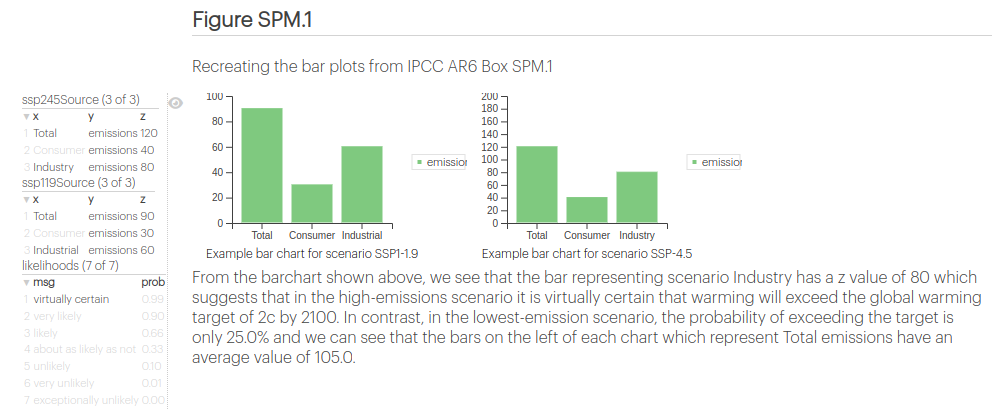
\includegraphics[width=0.9\textwidth]{fig/spm-figure-mockup-fluid.png}
   \caption{Prototype of SPM example in fluid}
   \label{fig:figure-spm-fluid}
\end{figure}

\begin{figure}
   \tiny
   \lstinputlisting[language=Fluid]{listings/bar-chart.fld}
   \caption{Source code for \figref{figure-spm-fluid}}
\end{figure}



Applying language models to the task of code generation is not new, however the aim of generating code that
itself produces natural language appears to be a novel one. We currently anticipate the following challenges,
and will add more as the work progresses.

\paragraph{Small number of examples:} as a language, Fluid is incredibly niche, and so we have a very small corpus
of programs on which to train a language model. Further, we currently only have 2 example programs that actually make
use of the \kw{LinkedText} construct which we intend to use. The problem then is how to best make use of the capabalities
of current language models in this context. For example, should we perform some sort of few-shot learning or prompt-engineering
technique on a large pre-trained model, should we augment our corpus of training examples manually or both? If we take a meta-learning
perspective (\todo{CITE}), we may run into problems of the model preferring syntax and function names from the languages we use to
train the model.

\paragraph{Counter-intuitive dependency relation:} at the moment, dependencies that are computed by Fluid can be counter-intuitive.
Until we revamp the underlying dependency model, we will need to generate code that follows the pattern of ``consuming'' input
data in order to produce the output text. This may be a problem for things like generating direct references to visual elements.

\paragraph{Potentially complex code:} for many purposes, we want to store the data objects being referred to in variables. This 
could mean complicated code, and cluttering a source file. We will potentially need to find a general pattern for this sort of thing,
so that an authors document doesn't get filled with extraneous variable declarations. 